\thispagestyle{quantoannone}
\pagestyle{quantoan}
\everymath{\color{quantoan}}
\graphicspath{{../quantoan/pic2/}}
\blfootnote{\color{quantoan}$^*$Lược dịch theo: https://mathshistory.st-andrews.ac.uk/Biographies/De\_Giorgi/ và Ennio de Giorgi -- Wikipedia.}
\blfootnote{\color{quantoan}$^1$Đại học Sư phạm Hà Nội.}
\begingroup
\AddToShipoutPicture*{\put(0,616){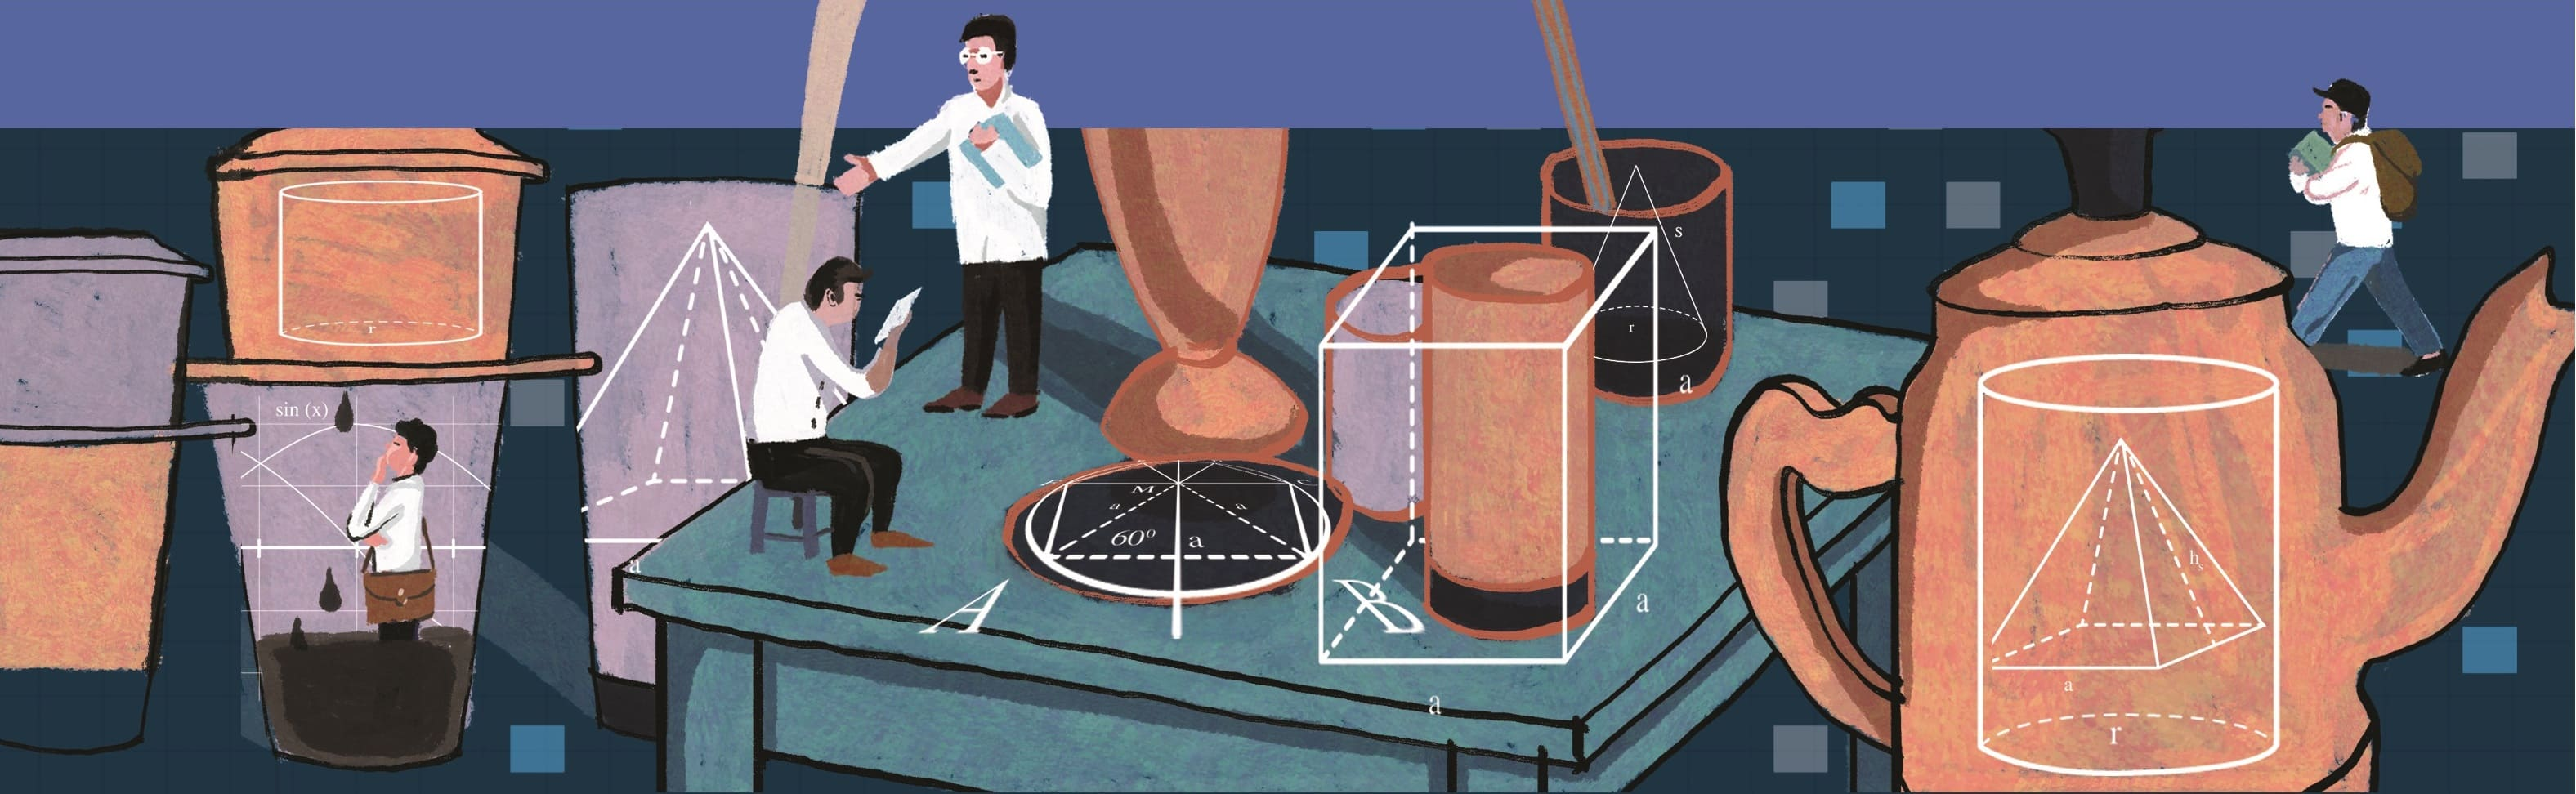
\includegraphics[width=19.3cm]{../bannerquantoan}}}
\AddToShipoutPicture*{\put(114,525){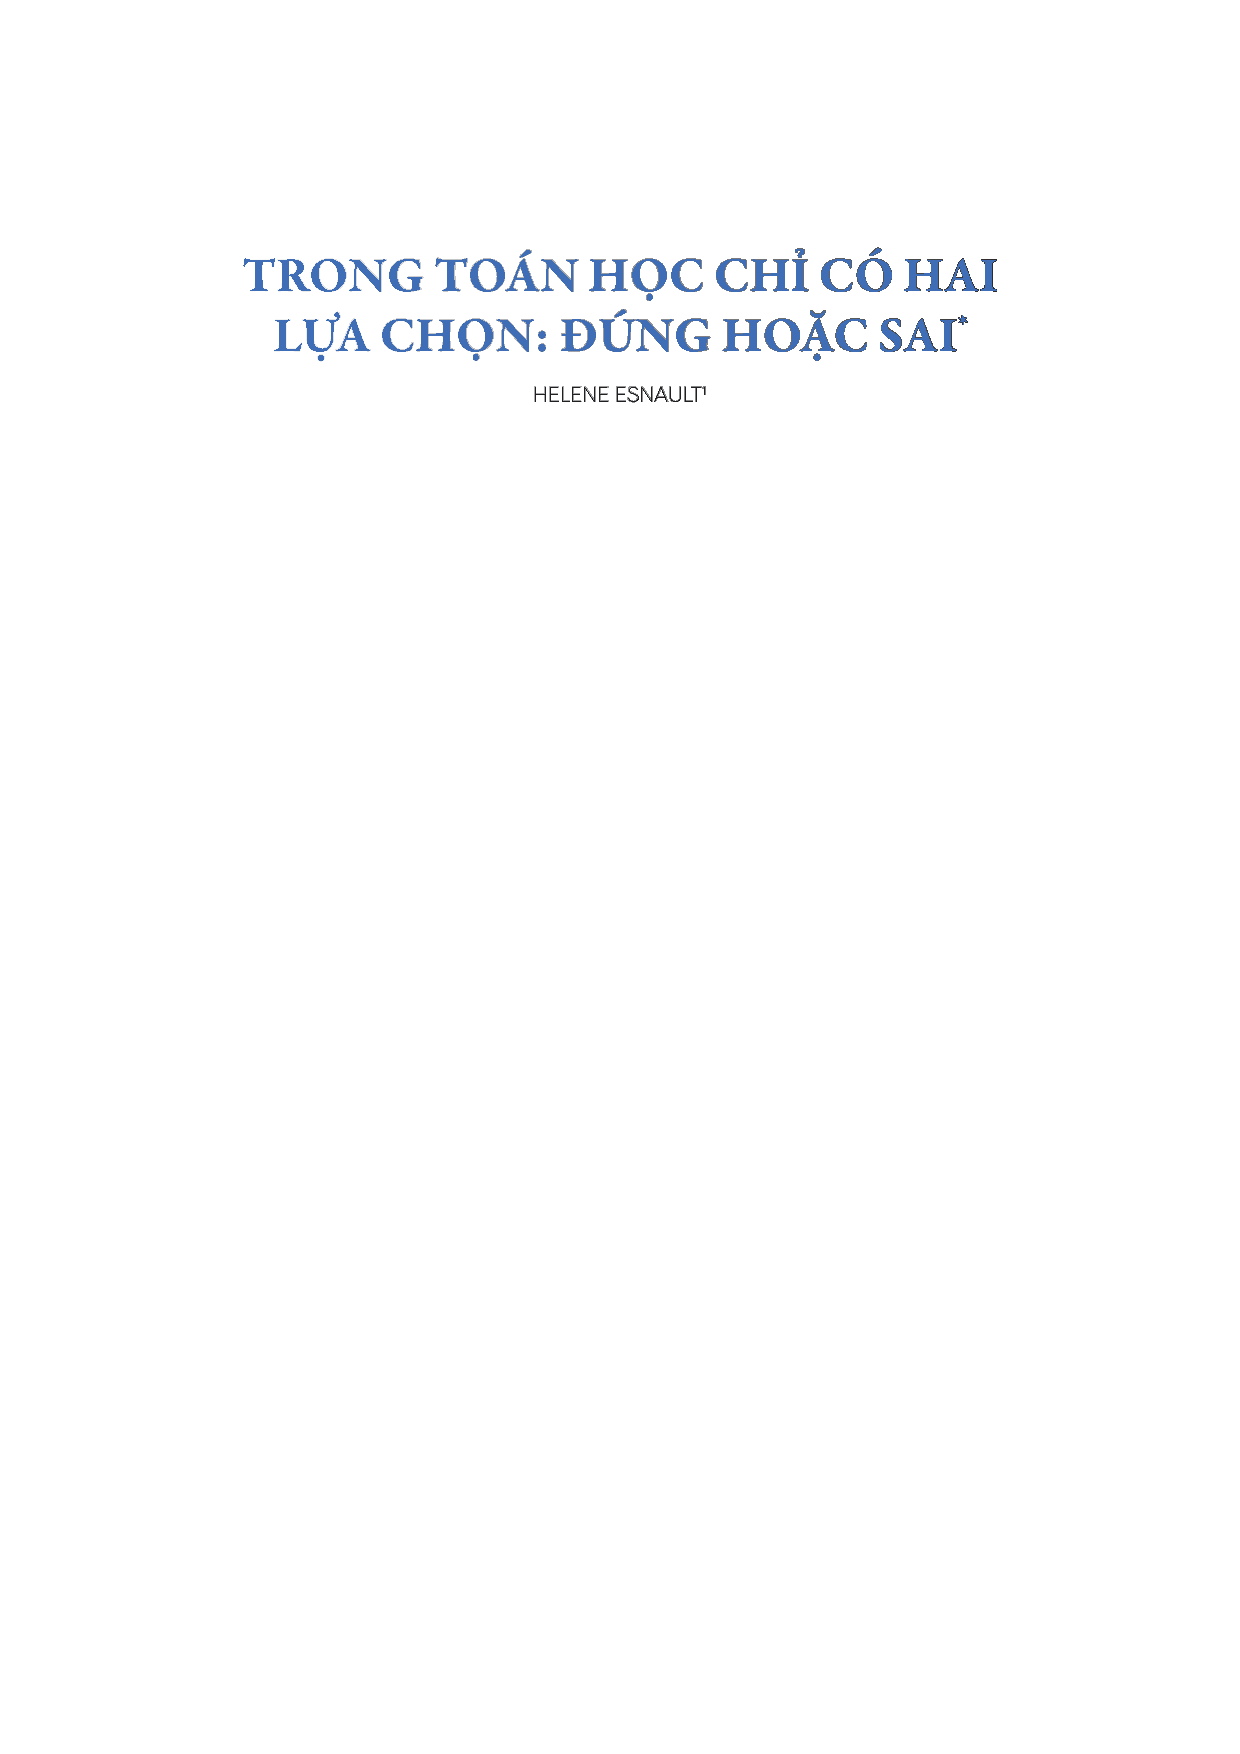
\includegraphics[scale=1]{../tieude.pdf}}}
\centering
\endgroup
\vspace*{180pt}

\begin{multicols}{2}
	Ennio de Giorgi $(1928-1996)$ là một nhà toán học người Ý, người đã nghiên cứu các phương trình đạo hàm riêng và các nền tảng của toán học. Ennio theo học tại trường trung học ``G. Palmieri' ở quê nhà và bộc lộ những tài năng đặc biệt. Tuy nhiên, lúc ban đầu, mối quan tâm của ông không hướng tới toán học [$1$]:
	\vskip 0.01cm
	\begin{wrapfigure}{l}{0.45\linewidth}
		\vspace*{-10pt}
		\centering
		\captionsetup{labelformat= empty, justification=centering}
		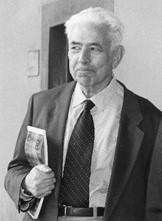
\includegraphics[width= 1\linewidth]{1}
		\caption{\small\textit{\color{quantoan}Ennio de Giorgi.}}
		\vspace*{-15pt}
	\end{wrapfigure}
	\textit{... khi còn nhỏ, tôi có sở thích đặc biệt trong việc mầy mò tìm ra lời giải cho những bài toán nhỏ, nhưng tôi cũng có niềm đam mê nhất định với việc thử nghiệm các thiết bị nhỏ -- các thí nghiệm, nếu không phải là của vật lý, thì là của thứ gọi là ``tiền vật lý".}
	\vskip 0.1cm
	Sau khi tốt nghiệp trung học năm $1946$, ông đến Rome để vào Đại học tại thủ đô, nhưng do đam mê các thiết bị, ông đã nhập học tại Khoa Kỹ thuật với ý định lấy bằng kỹ sư. Bất chấp việc quyết định chọn chủ đề nghiên cứu, De Giorgi đã khám phá ra niềm vui lúc đi học khi tìm ra cách chứng minh các định lý toán học khác với những chứng minh được viết trong sách giáo khoa. Đây chắc chắn là dấu hiệu ban đầu cho thấy tình yêu nghiên cứu của ông. Sau một năm học, Ennio quyết định rằng toán học chứ không phải kỹ thuật mới là môn học của mình [$1$]:
	\vskip 0.1cm
	\textit{Vào thời đó, các khóa học về toán học, kỹ thuật và vật lý đều giống nhau trong hai năm đầu tiên. Chính trong năm đầu tiên đó, tôi đã nhận ra rằng năng khiếu bẩm sinh của mình, trên tất cả, là về toán học.}
	\vskip 0.1cm
	Trong môn toán, De Giorgi theo học với Mauro Picone, người đã ảnh hưởng mạnh mẽ đến mình [$1$]:
	\vskip 0.1cm
	\textit{... tại Viện Toán học ở Rome, tôi đã học cùng và nhận bằng từ Giáo sư Picone, người với tư cách là một học giả, luôn trung thành với phong cách ``quý tộc" của những ngày đó, nhưng đồng thời là cũng là một người, trong thảo luận về các vấn đề khoa học, đã luôn hoàn toàn cởi mở. Tôi nhớ ông đã nói: ``Hãy nhớ rằng khi chúng ta nói về các vấn đề khoa học, bạn hoàn toàn có quyền nói với tôi rằng tôi đã nhầm, bởi vì chúng ta bình đẳng trước khoa học." Vì vậy, ông cực kỳ phóng khoáng trong đối thoại khoa học nhưng hoàn toàn tôn trọng kỷ luật và phong tục học thuật thời đó.} 
	\vskip 0.1cm
	De Giorgi hoàn thành chương trình học đại học vào năm $1950$ khi ông được nhận bằng tốt nghiệp. Sau đó, ông bắt đầu công việc nghiên cứu tại Viện Castelnuovo ở Rome, nơi ông là trợ lý cho Mauro Picone. Jacques--Louis Lions và François Murat viết trong [$4$] (xem thêm [$3$]):
	\vskip 0.1cm
	\textit{Vị Giáo sư và anh sinh viên đó thực sự là một sự kết hợp kỳ lạ: một người là người theo chủ nghĩa cổ điển, ăn mặc nghiêm túc và sang trọng; người kia, không chính thống, luôn đội xùm xụp chiếc mũ nồi kỳ khôi của mình. Nhưng M. Picone, một nhà quan sát dày dạn kinh nghiệm về sự phát triển của khoa học, đã biết cách phát hiện tài năng; ông ấy sớm thừa nhận khả năng đặc biệt của E. De Giorgi. Người trợ lý trẻ được giải phóng khỏi mọi ràng buộc và làm việc theo ý mình một cách nhàn nhã, nhưng cuối cùng lại hiệu quả đến kinh ngạc.}
		\begin{figure}[H]
		\vspace*{-5pt}
		\centering
		\captionsetup{labelformat= empty, justification=centering}
		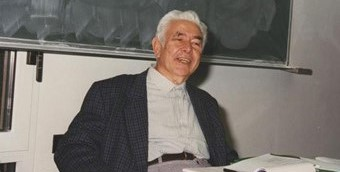
\includegraphics[width= 1\linewidth]{2}
		%		\caption{\small\textit{\color{}.}}
		\vspace*{-15pt}
	\end{figure}
	De Giorgi tham dự các bài giảng của Caccioppoli về lý thuyết độ đo hình học, nhưng vào thời điểm này ông đã có những ý tưởng của riêng mình về cách giải quyết các vấn đề về mặt cực tiểu. Dưới ảnh hưởng của các phương pháp mà Caccioppoli đã phát triển, De Giorgi tiếp tục phát triển các kỹ thuật mới trong lý thuyết độ đo hình học và ông áp dụng kết quả của mình vào phép tính biến phân để chứng minh định lý chính của ông cho hầu hết các mặt cực tiểu. Công trình đầu tiên của De Giorgi trong lý thuyết độ đo hình học về chủ đề các tập có chu vi hữu hạn mà ông gọi vào năm $1958$ là tập hợp Caccioppoli, theo tên người thầy và người bạn của mình. Định nghĩa của ông, áp dụng một số công cụ giải tích quan trọng và định lý De Giorgi cho các tập hợp, đã thiết lập một công cụ mới cho lý thuyết tập hợp cũng như các công trình của riêng ông. Thành tựu này không chỉ mang lại cho Ennio sự công nhận ngay lập tức mà còn thể hiện khả năng giải quyết các vấn đề bằng cách sử dụng hoàn toàn các phương pháp mới và hiệu quả, mặc dù đã được hình thành trước đó, nhưng có thể được sử dụng với độ chính xác cao hơn như  đã được thể hiện trong các công trình nghiên cứu của ông. Công trình sớm nhất  của ông nhằm mục đích phát triển một lý thuyết về tính chính quy cho các siêu  mặt cực tiểu, đã vĩnh viễn thay đổi cách chúng ta nhìn nhận lý thuyết cao cấp về các bề mặt cực tiểu và phép tính biến phân. Cùng với Enrico Bombieri và Enrico Giusti, ông đưa ra lời giải cho bài toán Bernstein về  mặt cực tiểu cho số chiều $n= 8$  vào năm $1969$, nhờ đó Bombieri được trao Giải thưởng Fields  vào năm $1974$.
	\vskip 0.1cm
	Năm $1955$ De Giorgi đã đưa ra một ví dụ quan trọng cho thấy tính không duy nhất nghiệm của bài toán Cauchy đối với các phương trình đạo hàm riêng dạng parabolic có các hệ số thỏa mãn các điều kiện chính quy nhất định. Trong năm tiếp theo, ông đã chứng minh được điều ngày nay mang tên ``Định lý De Giorgi" liên quan đến tính liên tục Hölder của nghiệm của phương trình đạo hàm riêng dạng elliptic cấp hai. Những kết quả này cũng tương tự với những kết quả được Nash chứng minh vào cùng một thời điểm. De Giorgi nói:
	\vskip 0.1cm
	\textit{Nash và tôi đã chứng minh cùng một định lý, hay nói đúng hơn là hai định lý rất gần nhau. Từ định lý Nash người ta có thể suy ra nhiều hay ít ngay lập tức định lý của tôi, theo một cách chứng minh hoàn toàn khác. Do đó, theo kinh nghiệm của tôi, việc khám phá một định lý có thể được thực hiện bởi những người khác nhau, như thể nó đã ở đó sẵn để chờ ai đó khám phá ra nó, và phát biểu của định lý đó sẽ luôn giống nhau. Tuy nhiên, phép chứng minh được sáng tạo ra có thể sẽ khác nhau rất nhiều tùy theo nhà toán học tìm ra nó.}
	\vskip 0.1cm
	Năm $1958$ De Giorgi được bổ nhiệm làm Trưởng khoa Giải tích Toán học tại Đại học Messina và ông đã nhận nhiệm vụ vào tháng $12$ năm đó. Tuy nhiên, ông giữ chức vụ này chưa đầy một năm vì đã được Alessandro Faedo tiếp cận, người đã thuyết phục ông chuyển đến Scuola Normale Superiore tại Pisa. Vào mùa thu năm $1959$ De Giorgi chuyển đến Pisa để đảm nhận chức vụ Trưởng khoa Giải tích Toán học.
	\vskip 0.1cm
	\textit{Trong gần bốn mươi năm, ông sống ở đó, dạy học ở đó và luôn là nguồn cảm hứng thường xuyên cho ngôi trường toán học mà ông thành lập. Luôn vui vẻ, luôn sẵn sàng, ông thích những cuộc tranh luận kéo dài với các học trò của mình, trong đó ông sẽ đưa ra những ý tưởng độc đáo và đề xuất những phỏng đoán hoặc phác thảo những dòng chứng minh.}
	\vskip 0.05cm
	De Giorgi đã nhận được nhiều sự tôn vinh vì những đóng góp toán học xuất sắc của mình, trong đó có Giải Caccioppoli năm $1960$, Giải thưởng Quốc gia của Viện Lincei (Accademia dei Lincei, Italia) năm $1973$, và Giải thưởng Wolf (Israel) năm $1990$, bằng tiến sỹ danh dự về Toán học của Đại học Paris năm $1983$, và về Triết học của Đại học Lecce năm $1992$. Ông được bầu vào nhiều Viện hàn lâm bao gồm:  Viện Accademia dei Lincei, Viện Hàn lâm Khoa học Giáo hoàng (Pontifical Academy of Sciences), Viện Hàn lâm Khoa học Turin, Viện Khoa học và Văn học Lombard, Académie des Sciences ở Paris và Viện Hàn lâm Khoa học Quốc gia Hoa Kỳ.
	\vskip 0.1cm
	Bên cạnh những thành công trong toán học của ông. Ennio là một người có tín ngưỡng và thường nói về niềm tin của mình [$2$]:
	\vskip 0.1cm
	\textit{Sách Châm ngôn, một trong những cuốn sách cổ nhất của Kinh thánh,  có nói rằng Thông thái đã ở cùng Thượng Đế khi Ngài tạo ra thế giới và rằng Thông thái sẽ được tìm thấy bởi những người tìm kiếm và yêu mến nó. Toán học là một trong những biểu hiện quan trọng nhất của tình yêu dành cho Thông thái.}
	\begin{figure}[H]
			\vspace*{-5pt}
			\centering
			\captionsetup{labelformat= empty, justification=centering}
			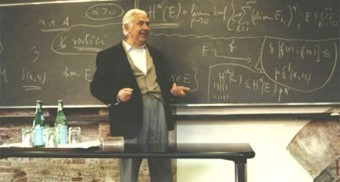
\includegraphics[width= 1\linewidth]{3}
			%		\caption{\small\textit{\color{}.}}
			\vspace*{-15pt}
		\end{figure}
	Ông cũng là một người nhiệt tình ủng hộ hòa bình và hữu nghị giữa các dân tộc và thể hiện điều này bằng những hoạt động tích cực của mình, ông phát biểu [$2$]:
	\vskip 0.1cm
	\textit{... bản Tuyên Ngôn Quốc Tế Nhân Quyền có Điều khoản nói về nền giáo dục khuyến khích không chỉ sự khoan dung mà còn cả sự hiểu biết và tình hữu nghị giữa các quốc gia khác nhau và các nhóm tôn giáo khác nhau. Hiểu biết và tình bạn là hai khái niệm thường bị lãng quên khi nói về lòng khoan dung. Sự khoan dung một cách trong sáng và đầy cảm tính là không đủ; chỉ khi được kết hợp với sự hiểu biết và tình bạn thì nó mới thực sự cho phép hoạt động của con người được phát triển. Đặc biệt, các ngành khoa học không thể tiến lên nếu không có sự hiểu biết và tình bạn giữa tất cả các nhà khoa học.}
	\vskip 0.1cm
	\textbf{\color{quantoan}Tài liệu tham khảo}
	\vskip 0.1cm
	[$1$]	L. Ambrosio, G. Dal Maso, M. Forti, M. Miranda and S. Spagnolo, Ennio De Giorgi (Italian), \textit{Boll. Unione Mat. Ital. Sez. B Artic. Ric. Mat.} ($8$) $2$ ($1$) ($1999$), $3-31$.
	\vskip 0.1cm
	[$2$]	M. Emmer (trs.), Interview with Ennio De Giorgi, \textit{Notices Amer. Math. Soc.} $44$ ($9$) ($1997$), $1097-1101$. \url{http://www.ams.org/notices/199709/emmer.pdf}
	\vskip 0.1cm
	[$3$]	J--L. Lions and F. Murat, Ennio De Giorgi ($1928-1996$) (French), \textit{Gaz. Math}. No. $71$ ($1997$), $30-34$.
	\vskip 0.1cm
	$[4]$	J--L. Lions and F. Murat, Ennio De Giorgi ($1928-1996$), \textit{Notices Amer. Math. Soc}. $44$ ($9$) ($1997$), $1095-1096$. \url{http://www.ams.org/notices/199709/murat.pdf}
\end{multicols}
\newpage
\begingroup
\AddToShipoutPicture*{\put(132,678){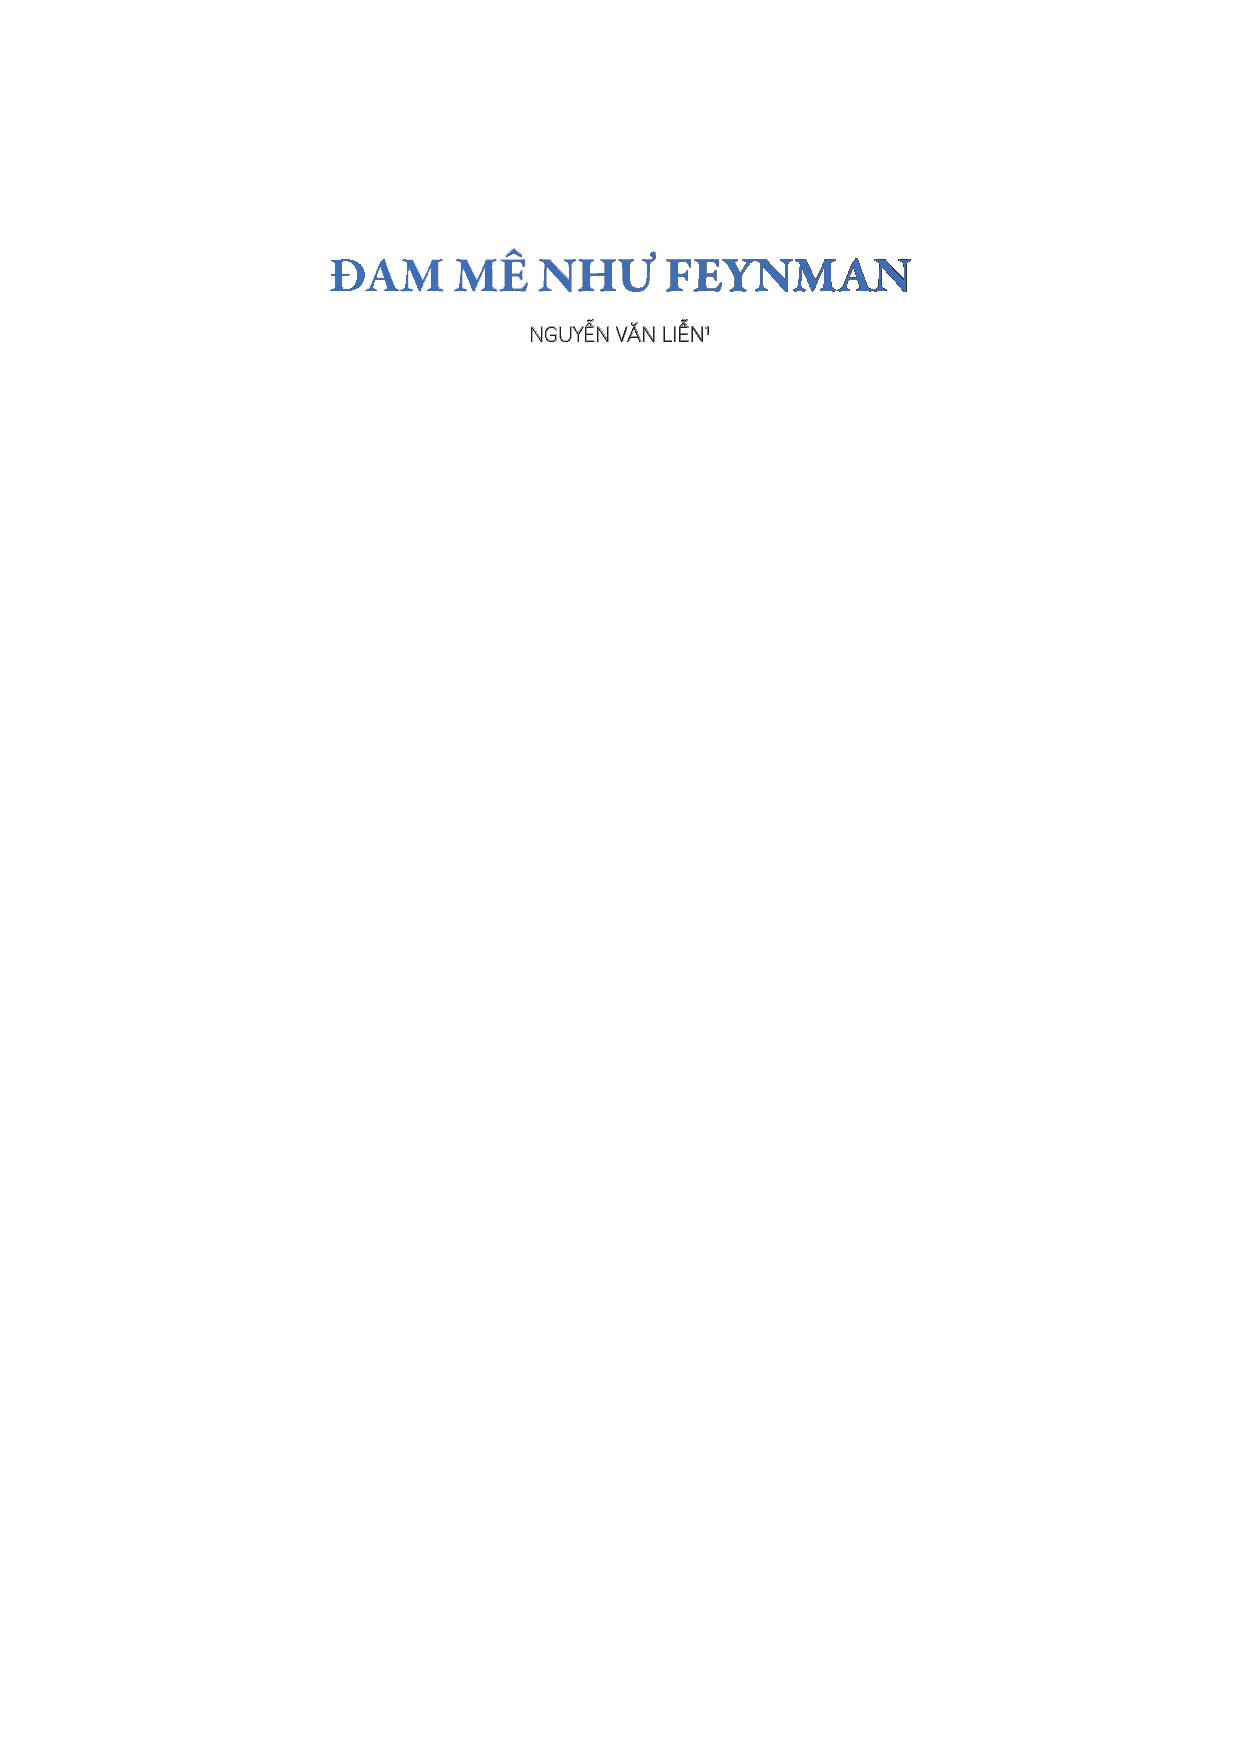
\includegraphics[scale=1]{../tieude2.pdf}}}
\centering
\endgroup
\blfootnote{$^1$\color{quantoan}Viện Vật lý.}
\vspace*{30pt}

\begin{multicols}{2}
	Richard Feynman ($1918-1988$, Mỹ) nổi tiếng là người trung thực không khoan nhượng và đam mê đến tận cùng. Về tính trung thực, người ta hay nhắc đến vụ ông trình diễn trực tiếp trên TV một ``thí nghiệm nhỏ", bỏ vòng cao su vào cốc nước đá, minh chứng rằng cao su mất tính đàn hồi ở nhiệt độ thấp, qua đó chỉ ra nguyên nhân dẫn đến thảm họa tàu vũ trụ con thoi ``Challenger", vạch trần chiến dịch tung hỏa mù của NASA về nguyên nhân của thảm họa này. Để công bố với người dân Mỹ sự thật ấy, Feynman đã phải vượt qua sức ép khủng khiếp từ các cơ quan công quyền Mỹ, trong đó có CIA và NASA. 
	\begin{figure}[H]
			\vspace*{-5pt}
			\centering
			\captionsetup{labelformat= empty, justification=centering}
			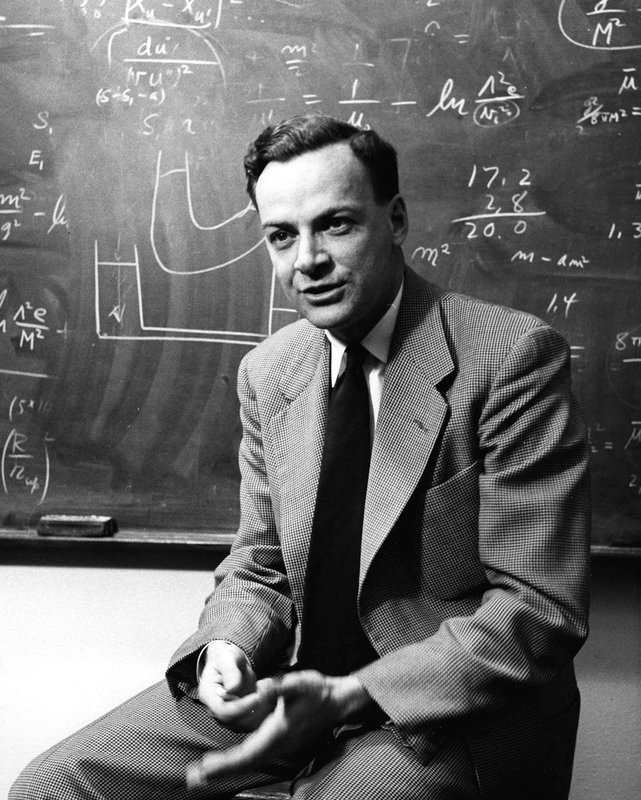
\includegraphics[width= 1\linewidth]{1a}
			\caption{\small\textit{\color{quantoan}Richard Feynman (ảnh từ bộ sưu tập của Viện Công nghệ California -- CalTech).}}
			\vspace*{-10pt}
		\end{figure}
	Feynman lắm đam mê. Đam mê vật lý, Feynman nhận giải Nobel Vật lý năm $1965$. Đam mê chơi trống, vở ba--lê do ông đệm trống nhận giải nhất trong cuộc thi ba--lê toàn nước Mỹ và giải nhì trong cuộc thi quốc tế tại Paris. Đam mê vẽ, ông đã có triển lãm tranh riêng. Không rõ ông biết những ngôn ngữ nào, chỉ biết thăm Brazil ông dạy bằng tiếng Bồ, thăm Nhật ông giao du bằng tiếng Nhật. Rồi có lần bạn bè định ``cho ông một vố", họ nhờ một cô Hoa kiều đón tiếp ông bằng tiếng Trung, Feynman đáp lại và cô ấy kêu trời, vì ông nói tiếng Quảng Đông, còn cô chỉ nói tiếng Bắc Kinh. Rất nhiều ``đam mê" kiểu như vậy được kể trong cuốn ``Feynman, chuyện thật như đùa" (NXB Trẻ) và hầu như tất cả đều có kết cục mỹ mãn, kiểu như giải Nobel. Có thể bạn nghĩ chắc ông này ``con nhà nòi", học ``trường quốc tế" từ nhỏ! Xin thưa, bố của Feynman là người bán rong bán quần áo, còn mẹ thì nội trợ. 
	\begin{figure}[H]
			\vspace*{-5pt}
			\centering
			\captionsetup{labelformat= empty, justification=centering}
			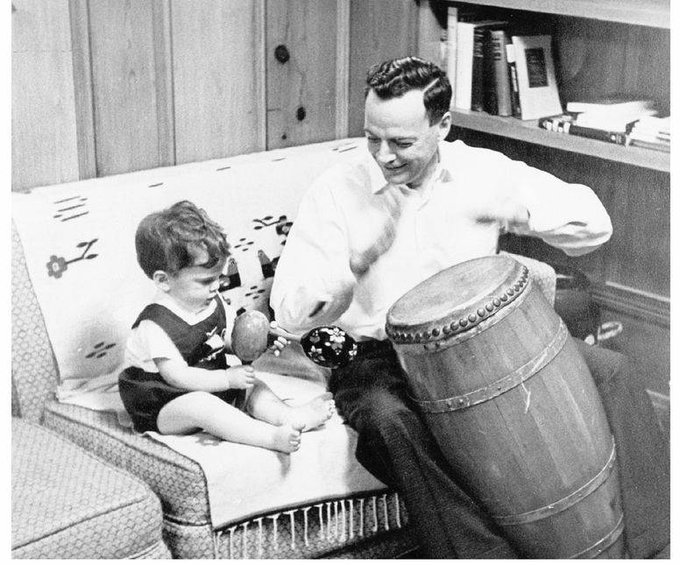
\includegraphics[width= 1\linewidth]{2a}
			\caption{\small\textit{\color{quantoan}Feynman chơi trống bên con trai (ảnh từ Internet).}}
			\vspace*{-10pt}
		\end{figure}
	Ông chơi trống bongo cực giỏi, nhưng chưa bao giờ học nhạc lý. Ông vốn vẽ rất kém, tự nhận chẳng thể vẽ nổi cái gì ngoại trừ cái kim tự tháp chỉ gồm mấy đường thẳng. Để học vẽ, Feynman ``đổi công" với một họa sỹ: ông dạy vật lý cho họa sỹ còn họa sỹ dạy vẽ cho ông. Hãy tưởng tượng một giáo sư nổi tiếng thế giới ngồi trong lớp vẽ cùng các cháu $8-9$ tuổi học cách gọt bút chì. Đam mê như thế chỉ có ở Feynman. Và, với ông đam mê chính là nguồn cội của thành công, chứ chẳng phải ``con nhà nòi" hay ``trường quốc tế" nào cả. Tiền bạc và chứng chỉ đầy người, mà không đam mê gì, thì làm sao có thành quả! 
	\begin{figure}[H]
			\vspace*{-5pt}
			\centering
			\captionsetup{labelformat= empty, justification=centering}
			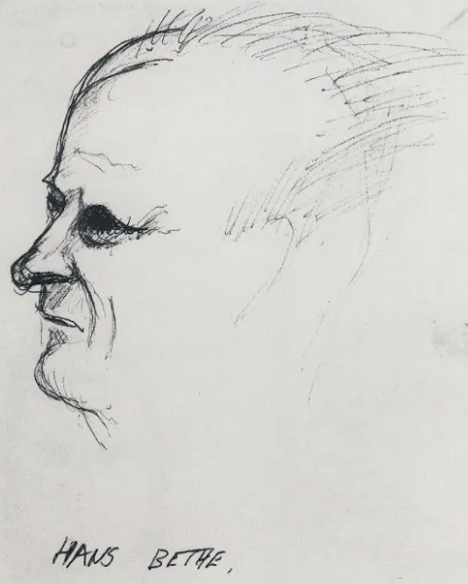
\includegraphics[width= 1\linewidth]{3a}
			\caption{\small\textit{\color{quantoan}Feyman vẽ Hans Bethe (giải Nobel Vật lý $1967$).}}
			\vspace*{-10pt}
		\end{figure}
	Duy có đam mê cuối cùng, Feynman đã không kịp nhìn thấy những gì mình muốn, trước khi về cõi vĩnh hằng. Đó là ``Cuộc phiêu lưu cuối cùng của Feynman"\footnote[2]{\color{quantoan}Xem thêm: Cuộc phiêu lưu cuối cùng của Feynman, in lần $2$, NXB Trẻ, $2023$.}. Cuộc phiêu lưu khởi đầu bằng một con tem có xuất xứ từ một nơi gọi là Tannu Tuva, mà Feynman có được từ khi còn nhỏ. Cái tên ``Tuva" xa lạ nằm yên trong đầu Feynman, cho đến một ngày hè $1977$ nó trở thành mục tiêu cho ``cuộc phiêu lưu" kéo dài hơn $10$ năm cuối của cuộc đời ông. Tôi cược là nhiều bạn chưa biết Tuva là địa danh nào và ở đâu. Để đỡ tra cứu, xin ``bật mí" ngay: đó là tên một quốc gia nhỏ nằm giáp phía Tây Bắc của Mông Cổ, vốn độc lập, nhưng đã sáp nhập vào Liên Xô cũ (và Nga ngày nay). Thủ đô của Tuva là Kyzyl. Tuva có gì đặc biệt mà khiến Feynman mê mệt đến vậy?
	\vskip 0.1cm
	Bạn có biết đâu là trọng tâm của châu Á (lục địa thôi chứ không tính các đảo)? Lấy tấm bìa cứng phẳng, vẽ lên đó bản đồ châu Á, cắt theo đường biên để được miếng bìa hình châu Á lục địa. Dùng một chiếc bút đầu nhọn chống phía dưới tấm bìa, di di đầu bút, để tìm vị trí mà tấm bìa nằm cân bằng trên chiếc bút thẳng đứng. Vị trí đó rơi vào Kyzyl, trọng tâm của châu Á. Tất nhiên, các nhà khoa học xác định điểm này bằng các phương pháp chính xác hơn, và ngày nay ở Kyzyl có tấm bia lớn khẳng định vị trí đặc biệt của thành phố này. Nhưng, chỉ chừng ấy thì không đủ để Feynman mất tới cả chục năm tìm cách tới thăm Tuva.
	\begin{figure}[H]
			\vspace*{-5pt}
			\centering
			\captionsetup{labelformat= empty, justification=centering}
			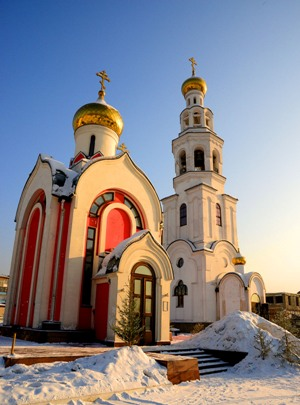
\includegraphics[width= 1\linewidth]{4a}
			\caption{\small\textit{\color{quantoan}Nhà thờ Phục sinh ở Kyzyl, Tuva (ảnh từ Internet).}}
			\vspace*{-10pt}
		\end{figure}
	Cái chính là ở quốc gia tí xíu bao bọc bởi những dãy núi cao ấy, thời gian gần như ngừng trôi: tất cả vẫn nguyên sơ như $500$ hay $1000$ năm trước. Thảo nguyên hoang dại. Những đàn tuần lộc hay bò Tây Tạng cũng dường như hoang dại. Cuộc sống du mục không thể tự nhiên hơn. Một nền văn hóa xa xưa và kỳ thú với kiểu hát hai giọng chỉ có ở Tuva, với thứ văn tự không thể tìm thấy trong bất cứ tự điển nào, với các tập tục rất lạ điều hành bởi các tù trưởng uy nghi và bí ẩn v.v. Tiếc là ít người biết Tuva, chứ không, người ta đã gọi quốc gia này là ``Thảo nguyên Xanh" cuối cùng của hành tinh Trái Đất (như Congo là Hành tinh Xanh cuối cùng). Đam mê Tuva, Feynman tìm đọc mọi tài liệu về Tuva, tìm hiểu văn tự Tuva, học cách hát của dân du mục Tuva, ăn mặc và trang trí như tù trưởng Tuva \ldots Và, nhất là, ông tìm mọi cách để có thể đến thăm Tuva.
	\vskip 0.1cm
	Đó là thời Chiến tranh Lạnh, lại nghe nói, gần Tuva có một cơ sở nghiên cứu bom nguyên tử, nên nơi đây là ``vùng cấm" với khách du lịch, nhất là khách nước ngoài. Thực ra, Viện Hàn lâm Khoa học Liên Xô sẵn sàng mời Feynman sang Moscow  đọc bài giảng rồi đi ``tham quan Kyzyl" theo kiểu mặc com--lê ở khách sạn có người bảo vệ v.v. Nhưng Feynman không thích như vậy, mà muốn tự mình mang ba--lô đến thảo nguyên, ngủ lều, uống sữa tuần lộc và hát hai giọng cùng dân bản xứ. Ấy thế cho nên ông mất cả chục năm tìm kiếm một giấy mời như mình muốn. Và, đầu tháng Ba $1988$, một giấy mời như thế đã gửi đến địa chỉ của Feynman, chỉ tiếc là hai tuần trước đó, vào ngày $15$ tháng Hai, ông đã ra đi mãi mãi, nên chỉ có thể trải nghiệm ``Cuộc phiêu lưu cuối cùng" của mình trong tâm trí và trái tim của những người ở lại. Không rõ, ở Thế giới bên kia Feynman đang đam mê gì?
\end{multicols}